% Sample file for the use of compsoft style file.
%
\documentclass{compsoft}
% \documentclass[L]{compsoft}
% \documentclass[S]{compsoft}
% \documentclass[S,L]{compsoft}
% \documentclass[K]{compsoft}
% \documentclass[K,L]{compsoft}
% \documentclass[U]{compsoft}
% \documentclass[U,L]{compsoft}

% Preamble
%
% 「コンピュータソフトウェア」誌に掲載される論文の場合,次で
% 巻数,号数,開始ページ,終了ページを指定する.
\volNoPp{29}{1}{78}{84}

% ワークショップによる推薦論文の場合,ワークショップ名を指定する.
% \suisen{ワークショップ名}

% 特集の場合,特集のタイトルを与える.
 \tokushu{実践的IT教育}

% 大会論文の場合,\taikai で開催年を指定する.ここで指定した年から
% 大会の回数は計算される.
% \taikai{2009}

% ここに,使用するパッケージを列挙する.
\usepackage[dvips]{graphics}
\usepackage{url}
\usepackage{color}
\usepackage{multirow}
\usepackage{listings,jlisting}
\usepackage{here}

% ユーザが定義したマクロなどはここに置く.ただし学会誌のスタイルの
% 再定義は原則として避けること.

\lstset{%
	language={R},
	basicstyle={\normalsize},%
  	identifierstyle={\normalsize},%
  	commentstyle={\normalsize\itshape},%
  	keywordstyle={\normalsize\bfseries},%
  	ndkeywordstyle={\normalsize},%
  	stringstyle={\normalsize\ttfamily},
  	frame={tb},
  	breaklines=true,
  	columns=[l]{fullflexible},%
  	numbers=left,%
  	xrightmargin=0zw,%
  	xleftmargin=3zw,%
  	numberstyle={\normalsize},%
  	stepnumber=1,
  	numbersep=1zw,%
  	lineskip=-0.5ex%
}

\makeatletter
\newcommand{\subsubsubsection}{\@startsection{paragraph}{4}{\z@}%
  {1.0\Cvs \@plus.5\Cdp \@minus.2\Cdp}%
  {.1\Cvs \@plus.3\Cdp}%
  {\reset@font\sffamily\normalsize}
}
\makeatother
\setcounter{secnumdepth}{4}

\begin{document}

% 論文のタイトル
\title{過去の情報を用いたPBL向け工数見積り手法の提案}

% 著者
% 和文論文の場合,姓と名の間には半角スペースを入れ,
% 複数の著者の間は全角スペースで区切る
%
\author{齋藤 尊 新美 礼彦 伊藤 恵
%
% ここにタイトル英訳 (英文の場合は和訳) を書く.
%
\ejtitle{Proposal of a Man-hour Estimation Method Using the Past PBL Data}
%
% ここに著者英文表記 (英文の場合は和文表記) および
% 所属 (和文および英文) を書く.
% 複数著者の所属はまとめてよい.
%
\shozoku{Takeru Saito, Ayahiko Niimi, Kei Ito}{公立はこだて未来大学大学院システム情報科学研究科}%
{Graduate School of Systems Information Science, Future University Hakodate}
%
% 出典情報は \shutten とすれば出力される.
\shutten
%
% 受付年月日,記事カテゴリなどは自動的に生成される.
\uketsuke{2017}{3}{31}
%
% その他,脚注に入れるものがあれば,\note に記述する.
%\note{脚注に入れる内容}
}

%
% 和文アブストラクト
\Jabstract{%
本研究では,学生主導で実施されるソフトウェア開発PBL(Project-Based Learning)のマネジメント支援を目的とする.
ソフトウェア開発経験の浅い学生がプロジェクトを管理するPBL では,学生の経験不足などが原因で工数見積りの誤りが発生し易い.
一般的なソフトウェア開発では,開発工数を見積る手法を利用するが,データ収集とモデル構築・工数計算をプロジェクト進行中に行う必要があるため,学生が利用するのは難しい.
一方PBL ではプロジェクト管理ツールなどから様々な開発データを収集できるが,それらは十分に活用されていない.

そこで本研究ではCoBRA法をベースにした工数見積り手法を提案する.
この手法では過去に実施されたPBLの開発データを利用することによって,実施中のシステム開発PBLの成果物作成に要する工数を見積る.
本研究では見積り精度の評価とPBL参加学生へのアンケートを実施するため,進行中のPBLへの適用実験を行った.
またこの適用実験では,データ収集の簡便化のためプロジェクト管理ツール運用ルールを設定した.
%しかしこのアンケートの結果,運用ルールが遵守されていないことが確認できた.
%この適用実験で算出した見積り工数をPBL参加者に公開し,その見積り結果の感想もアンケートによって収集したが,多くの参加者が見積り結果を有効に活用できていなかった.
%だが本研究の見積り及びプロジェクト管理ツールの運用ルールによって,「要件の見直ができた」や「開発スコープの訂正に役立てることができた」などの意見も得ることができた.
}
%
% 英文アブストラクト(本サンプルの原論文にはなし)
\Eabstract{
 In this study, it is purpose that we support students to manage their PBL(Project-Based Learning). 
In PBL which students manage, delay of schedule and temporary tasks are easy to happen because of immature man-hour estimation. 
In a general software development, project members use man-hour estimation methods.
But, it is difficult that participants use these estimation methods because they are busy to develop software.
On the other hand, much data can be collected in PBL. However, it has not been used enough. 

So, we propose the estimation method which is based on CoBRA(Cost estimation, Benchmarking and Risk Assessment). 
This method uses past PBL data and calculates man-hour it takes to implement their system.
In this study, we conducted the experiment targeting PBL in progress in order to take a survey from participants.
%To do this experiment, I decided operation rule of project management tools.
%But, in the result of survey, some participants did not adhere to the operation rules.
%I announced their estimation man-hour and took a survey but many of them could not fully utilize these estimation results.
%However, I found the advantage of that participants can use estimation results to review the development scope.
}
%
\maketitle

\section{序論} % 章のタイトル
%\section{Introduction} % sample of English style


% \includegraphics[width=??cm]{hoge.eps} % 図(EPS形式)を読み込む場合

\subsection{背景} \label{Background}% sectionのタイトル
% 以下に背景,関連する環境,状況,技術に関する概要を記述.
近年,実践的なソフトウェア開発教育手法の一つとしてPBL(Project-Based Learning) が注目されている.
PBLでは学習者がチーム内の意思決定に基づき,問題発見・問題解決を行うことを重視した教育手法である\cite{pbl}.
特にソフトウェア開発の分野では学習者が上流工程からソフトウェア開発を経験する場合が多い.
これは実際の社会が抱える問題に対する解決アプローチを経験できるという点で,特に注目されている.
PBL によるソフトウェア開発は企業が事業として行う開発とは異なり,学習者がプロジェクトマネジメントや開発ツールの利用方法・開発言語を学びながらソフトウェアを開発する.
そのため開発技術の不足から,プロジェクトのスケジュール遅延が発生しやすいと考えられる.

またソフトウェア開発において計画的なプロジェクト運行には,対象開発物への正確な開発工数の見積りが必要である.
そのため,数学的な見積りモデル手法が複数提案されている.
しかし,これらの手法は一定の知識や経験がなければ有効な利用が難しい.
そのため,特に学生がプロジェクト管理を行うPBLでは利用が難しい.

\subsection{研究目標} \label{Parpose}
本研究では,PBLでは通常のソフトウェア開発と同様に複数の開発データを収集することができることに着目し,大学等の教育機関で保存している過去のPBL実績データを利用して進行中のPBLで行われるソフトウェア開発に要する工数を見積る手法を提案する.
本手法はPBLに参加する学生が利用することを想定し,既存のプロジェクト管理ツールなどから収集できるデータのみを見積りに用いることで,PBL参加者に大きな負担をかけずに工数見積りを行うことを目指す.

また提案手法を評価するため,進行中のPBLを対象とした見積り実験を実施する.
ここで算出した見積り結果を当該プロジェクトに開示し,見積り結果へのアンケート調査を行う.

%--------------------------------------------------------------------
\section{関連研究} \label{Other-study}
%本章ではPBLと工数見積りに関する先行研究について紹介する.

\subsection{PBLで発生する問題} \label{occurred-problem}
永田らの大学院で実施されたPBL では,スケジュール遅延などの問題が複数発生したことがわかる\cite{nagata2011}.
この報告ではWBS(Work Breakdown Structure)によって実際の作業内容とその完了にかかる時間の見積りを行っていた.
しかし,この見積りが正確に行えず,実際の工数との差異が大きくなったと報告している.
この問題への対策として,直近の作業となるごとに詳細に予定工数を設定するローリングウェーブ計画法を提案している.
しかし,この報告では直近の予定工数しか精密に見積りが行えないため,順次見積りを行わなければならず,PBL参加者への作業量を増加させる問題がある.
BPLは一般的に人員の増加がなされず,作業工数の増加がスケジュール遅延に直結する,
そのため,PBLのスケジュール遅延にならないよう,極力作業工数を増やさない見積り手法が必要である.

%\subsection{PBLのマネジメント支援の試み} \label{PBL-manage}
%スケジュール遅延以外にも,PBL では独自の評価方法の必要性や参加者ごとに実行環境が違うため発生するトラブルなど,課題点が未だ複数存在する.
%松澤らはEVM(Earned Value Management) を用いることで,数値データに基づいた評価方法を提案している\cite{mastuzawa2009}.
%これは時間をコストと設定した上で,PBL参加者にデータ収集とEVMによるプロジェクト評価を行った.
%このマネジメント支援の試みでは既に完了したプロジェクトの実績データを利用してはいない.
%そのため,蓄積したデータを十分に活用したマネジメント支援の仕組みが必要であると考えられる.

\subsection{見積り手法} \label{estimation-method}
ソフトウェア開発における工数見積りは一般的に過去の類似プロジェクトの実績を参考に見積る類推法や専門家による判断,プロジェクト特性を説明変数として用いて工数を見積るパラメトリック法がある

\subsubsection{ファンクションポイント法} \label{fp}
ソフトウェア開発における工数見積りを行う場合,開発対象の開発規模を推定することが必要である場合が多い.
開発規模の代表的な指標としてファンクションポイント(FP)がある\cite{FP}.
FPは上記区分ではパラメトリック法に属する方法で導出されるが,この手法は開発工数そのものではなく,開発対象の規模を算出する.

\subsubsection{説明変数を用いる工数見積り手法} \label{parametrix}
ソフトウェア開発プロジェクトには,開発規模だけでなく開発環境や開発にあたって遵守しなければならない条件,参加メンバーの習熟度など複数の要因が工数に影響を与える.
そのため説明変数を用いて工数を算出する場合,FPだけでなくそれらの要因を説明変数として利用しなければならない.
この説明変数には開発規模やプロダクト,人材に関するメトリクスなどが一般的に必要とされている\cite{ipa-web}.
これらの説明変数のうちいずれを利用するかは見積り手法やプロジェクトによって変わる.
%天嵜らは5種類の変数選択手法を比較し,性能に関する評価を行った\cite{amasaki2006}.
%この変数選択は予測精度向上のみならず,見積りモデルを単純にすることができる.
%天嵜らの研究ではステップワイズ法による変数選択が最も良い結果を与えたと報告しているが,同時に一般性を主張するには別のデータセットを用いた実験を行わなければならないとしている.

\subsection{PBLを対象とした工数見積り} \label{PBL-estimation}
PBL を対象とした見積り手法に関して八島らはユースケースポイント(UCP) 法による見積りの検証を行っている\cite{yashima2011}.
この研究では計画段階で作成されたユースケースでは見積り精度が悪いという問題点がある.
UCP法はFP法と同様,開発規模や作業量だけの算出であるため,工数見積りに直接利用するには不十分である.

%--------------------------------------------------------------------
\section{提案する見積り手法} \label{Proposed-method}
本研究では過去に実施されたPBLの実績データを利用し,見積りモデルの構築と見積り結果の算出を行う.
そのため,CoBRA法を元にした工数見積り手法を提案する.
本章ではまずCoBRA法について述べ,その後,提案手法について述べる.

\subsection{CoBRA法} \label{CoBRA}
CoBRA法(A Hybrid Method for Cost Estimation, Benchmarking, and Risk Assessment)とは,説明変数を用いる見積り手法のうち,過去に実施されたソフトウェア開発の定量的データとソフトウェア開発熟練者の経験をもとに見積りを行う手法である\cite{CoBRA}.
CoBRA方では以下3つを前提条件としている.

\begin{enumerate}
\setcounter{enumi}{0}
	\item ソフトウェア開発熟練者は開発コストを,経験をもとに定量的に把握できる.\label{expart}
	\item 純粋状態において工数と開発規模は比例する.\label{linary}
	\item 開発における諸要素によって,工数と開発規模の線形関係に振れが生じる.\label{CO}
\end{enumerate}	

前提条件\ref{CO}より,開発期間に影響を与える要素を工数変動要因と呼ぶ.
この工数変動要因は$ {\it CO_{i} } $と表す.
また工数変動要因による工数への影響が全く無く,前提条件\ref{linary}のみが見積り結果に現れる状態を本研究では純粋状態と呼ぶ.

このCoBRA法では過去のプロジェクト実績データを利用し,見積りモデルを構築するため本研究の目的に適している.
しかし,PBLではCoBRA法のモデル構築に必要な見積り熟練者の協力を得ることが難しい.
そのため,本研究では見積り熟練者の協力がなくても見積りモデルが構築できるよう,CoBRA法を改変した手法を提案する.

\subsection{提案手法} \label{proposed}

\ref{CoBRA}節より,見積り熟練者の協力を得ずに見積りが可能となるよう,通常のCoBRA法の前提条件3つに加えて以下2つを前提条件に追加する.

\begin{enumerate}
\setcounter{enumi}{3}
	\item 見積り対象プロジェクトが開発期間中に予想した開発工数は純粋状態の見積り結果と一致する.\label{expected}
	\item $ {\it CO_{i} } $は当該工数変動要因の取得値と,実績工数を利用して算出した重回帰係数の積に比例する.\label{coeff}
\end{enumerate}

前提条件\ref{expected}はPBL参加者は工数見積りの際,工数変動要因を考慮できていないことが多いため設定した.
この前提条件\ref{coeff}により,前提条件\ref{expart}の開発熟練者の協力がなくとも ${\it CO_{i} } $の値を収集データからのみ算出できる.

これらの条件を踏まえ,本研究では以下の見積りモデルを提案する.

\begin{equation}
{\it PM = \alpha \times Size} \times ( 1 + \beta \times \sum ({\it Data_{i}} \times {\it Coeff_{i} }) ) \label{proposed-model}
\end{equation}

式\ref{proposed-model}の${\it PM}$は算出する見積り工数を表し,${\it Size}$は開発規模を表している.
また各工数変動要因の取得値が${\it Data_{i} }$,その重回帰係数が${\it Coeff_{i}}$である.
${\it Data_{i} }$に該当する数値として,プロジェクト参加人数などがある.
加えて${\alpha }$は開発規模1単位あたりの必要工数,$ \beta $が$ {\it Data_{i}} \times {\it Coeff_{i}}$ を工数変動要因の影響率とするための調整定数である.

この見積りモデルによって見積りを行う際には,まずモデル構築によってパラメータ$ \alpha $,$ {\it Coeff_{i}} $を設定する.
その後,見積り対象のプロジェクトのデータを収集し,当該プロジェクトの開発規模及び各工数変動要因の取得値を$ {\it Size} $,$ {\it Data_{i}} $に代入し計算する.
この見積り手法では当該プロジェクトが開発するシステムの実装期間を見積り結果として出力する.
ここで算出する見積り結果は実際に開発を行っている時間ではなく,開発を行っていない時間も含めた工数を意味している.
これはPBLに参加する学生は演習時間外にもPBL活動を行っており,学生の作業負担を増やさずに正確な作業時間を計測することは困難であることが理由である.

\subsubsection{モデル構築手順} \label{model-const}
式\ref{proposed-model}は以下の手順で構築する.

\begin{enumerate}
\item データ整形 \label{proposed-step1} \\
収集した各データのうち,欠損値はその欠損部分に0を代入する.
また全プロジェクトで値が欠損している工数変動要因は,その要因自体をデータセットから除外する.

すべての工数変動要因を数値として利用するため,名義尺度に属する工数変動要因をダミー変数に変換する.
また多重共線性を排除するため,各工数変動要因間の分散拡大係数(${\it VIF} $)が10以上となる組み合わせのうち1種を除きすべて除外する.

\item $ \alpha $の算出 \label{proposed-step2} \\
\ref{proposed}節の前提条件\ref{expected}より,目的変数を$ {\it Expected} $,説明変数を${\it Size}$とした最小二乗法により定数$\alpha$を算出する.

\item $ {\it Coeff_{i} } $の算出 \label{proposed-step3} \\
手順\ref{proposed-step1}で整形した工数変動要因を元に,$ {\it Coeff_{i} } $の算出を行う.
実績工数を$ {\it Actual} $としたとき,前提条件\ref{CO}及び\ref{expected}より$ {\it Coeff_{i} } $は実績工数と当該プロジェクトの予想工数の差と等しい.
そのため以下の式\ref{step3-method}に対し目的変数を$ {\it Actual - Expected } $,説明変数を$ {\it Data_{i}} $とした重回帰分析を行う.
\begin{equation}
Actual - Expected = \sum Data_i \times {\it Coeff_i} \label{step3-method}
\end{equation}
この重回帰分析をもとに算出した標準化偏回帰係数を$ {\it Coeff_{i} } $に設定する.

\item $ \beta $の算出 \label{proposed-step4} \\
上記の手順によって算出した$ \alpha $,$ {\it Coeff_{i}} $を説明変数,${\it Actual }$を目的変数とした回帰分析を行う.
そこで得られた回帰係数を$ \beta $に設定する.
  
\end{enumerate}

\subsection{工数変動要因とその他見積り用パラメータの収集} \label{used-data}
\subsubsection{対象プロジェクト} \label{obj-project}
本研究では見積りモデル構築や見積り実験実施のため,著者ら所属大学で2013年から2015年に実施されたPBL29件からデータを収集した.
そのうち11件はおおよそ1週間程度の期間で実施される短期集中のPBLで,通常のPBLと異なり1日の講義時間枠のすべてを実施時間に利用するPBLであるため,\ref{enPiT-PBL}章の実験では残り18件のデータを見積りモデル構築に利用した.

\subsubsection{メトリクス} \label{metrix}
対象プロジェクトから工数変動要因を42種,その他見積り用パラメータを4種収集した.
モデル構築用パラメータとして予定工数やFP,工数変動要因としてプロジェクト参加者数やユースケース数,開発言語などを収集した.
これらは議事録やプロジェクト管理ツールの記録,ソースコード等から算出した.
収集したメトリクスの種類は\url{https://github.com/keilab2016/PBLEstimationTool/blob/master/palam-def.md},その収集結果は\url{https://github.com/keilab2016/PBLEstimationTool/blob/master/Teaching_data.csv}にて確認できる.
このメトリクスのうち,議事録等で記録されていないなどの原因でデータが欠損していた場合はNAを入力した.

%------------------------------------------------------------------------------
\section{進行中PBLへの適用実験} \label{enPiT-PBL}
本章では2016年度に実施されたPBLを対象とした見積り実験について述べる.

\subsection{実験概要} \label{enPiT-exp-summary}

\subsubsection{見積り対象PBL} \label{enPiT-PBL-detail}
この実験を行うため,2016年度にenPiTで行われたPBLのデータの収集を行った.
enPiTとは``大学間・企業間で連携を取りつつICTを用いた新たな価値創出ができる人材の育成''を行っている事業である\cite{enPiT2016}.
本研究ではenPiTにおいて著者ら所属大学で行われた分散PBL(図\ref{fig:enPiT})6チームのデータを見積り実験の対象とした.

\begin{figure}[tb]
\begin{center}
\scalebox{0.25}{ 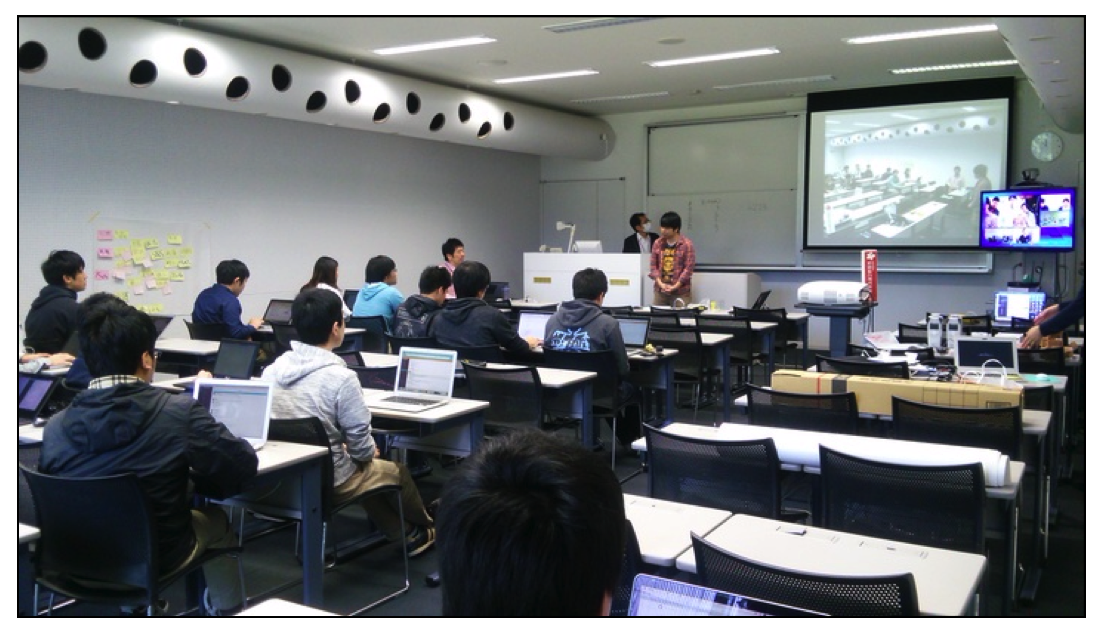
\includegraphics{enpit2016.eps}}
\end{center}
\caption{2016年度enPiT分散PBL}
\label{fig:enPiT}
\end{figure}

\subsubsection{実験準備} \label{enPiT-exp-preparation}

本研究はこのPBLの開始時点から,データ収集に向けた準備を行った.
このPBLではプロジェクト管理および構成管理のためにGitHubを利用している\cite{github}.
そこでこのGitHubからデータ収集を行った.
また本実験を実施するに当たって,必須データの確実な記録とデータ収集の簡略化のため,議事録フォーマットの利用やIssue発行に関するルールなどのGitHub運用ルールを設定した.
設定したGitHub運用ルールの詳細は\url{https://github.com/keilab2016/PBLEstimationTool/blob/master/Operational_rule.md}に記載する.
これらのGitHub運用ルールを設定することで,ルール設定を受けていないPBLに比べ,本研究で利用するデータを確実かつ容易に収集できるようになった.

\subsubsection{収集データ} \label{enPiT-data}
収集できたデータは\url{https://github.com/keilab2016/PBLEstimationTool/blob/master/2016_enPiT.csv}にて確認できる.
表\ref{data-example}は収集データの抜粋である.
\begin{table}[ht]
\caption{収集データ例}
\label{data-example}
\centering
\scalebox{0.9}{
\begin{tabular}{r | r | r | r | r}  \hline
 & Estimated & Actual & FPTrial & FPApproxi \\  \hline
a & 144 & 116 & 330 & 103 \\  \hline
b & 216 & 126 &  85 &  44 \\  \hline
c & 144 & 172 & 135 &  67 \\   \hline
\end{tabular}}
\end{table}

%収集データのうち,プロジェクト2016\_aはIssueに設定した予定実装期間と参加人数から${\it Estimated}$は144となり,議事録中の実装予定機能の一覧から${\it FPTrial}$は330となった.
%その他の工数変動要因のうち,すべてのIssueに重要度に関するLabelが設定されていなかったため${\it Importance}$は2.00を設定した.

\subsection{実験結果と考察} \label{enPiT-exp}
\ref{enPiT-data}節のPBLデータを用い,見積り実験を行った.
また見積りにおいて,\ref{obj-project}節のデータを見積りモデル構築に用いた.
モデル構築のため手順\ref{proposed-step1}のデータ整形を行った結果,18種の工数変動要因が見積りに適用された.

この見積り結果が表\ref{enPiT-result}である.
\begin{table*}[htb]
\centering
\caption{適用実験の見積り結果}
\label{enPiT-result}
\scalebox{0.8}{
\begin{tabular}{c | r | r | r | r | r | r} \hline
プロジェクト & a  & b & c & d & e & f \\ \hline
見積り工数(人日) & 436.4151 & 160.1002 & 185.6781 & 96.0558 & 234.4776 & 80.7914 \\ \hline \hline
実績工数(人日) & 116 & 126 & 172 & 140 & 210 & 175 \\ \hline
相対誤差(\%) & 276.2199 & 27.0637 & 7.9524 & -31.3887 & 11.6560 & -53.8335 \\ \hline 
\end{tabular}}
\end{table*}
ここで表\ref{enPiT-result}の見積り工数及び予想必要日数は全プロジェクトのデータ収集が完了した直後に算出し,実績工数及び相対誤差は全チームが開発対象システムの実装を終えて以降,データ収集と算出を行った.
表\ref{enPiT-result}のうち,プロジェクトaの見積り工数は436.4151人日となった.
表\ref{enPiT-result}の相対誤差平均は116.2700\%,中央値は9.8042\%となった.
この結果より,外れ値による見積り精度への影響が大きいことが確認できた.
特にプロジェクトaの相対誤差が非常に大きいが,これは参照ファイルの量によって開発規模に利用したFP値が実態よりも過剰に大きくなったことが原因と考えられる.

2016年11月25日に行われたPBL講義時間に,この表\ref{enPiT-result}の見積り工数及び予想必要日数を当該プロジェクトの参加者に伝えた.この時点でプロジェクトc,e,fはすでに実装開始から3週間以上が経過しており,その他は実装開始から2週間以内であった.

\subsection{アンケート調査} \label{quest}
本見積り結果に関してPBL参加者に対し,見積り結果と結果の開示時期及びGitHub運用ルールに関してアンケートを実施した.
このアンケートでは,発表した見積り結果を有用に活用できたのか,運用ルールにかかるコストがPBLで許容できるものであったかなどを調べるため実施した.

\subsubsection{アンケート項目と結果} \label{quest-detail}
アンケートを2016年12月9日に実施し,その結果29名中19名から回答を得られた.

設問1``お伝えした見積り結果はあなたの想像と比べてどうでしたか''の回答結果は図\ref{fig:q1}の通りである.
\begin{figure}[tb]
\begin{center}
\scalebox{0.25}{ 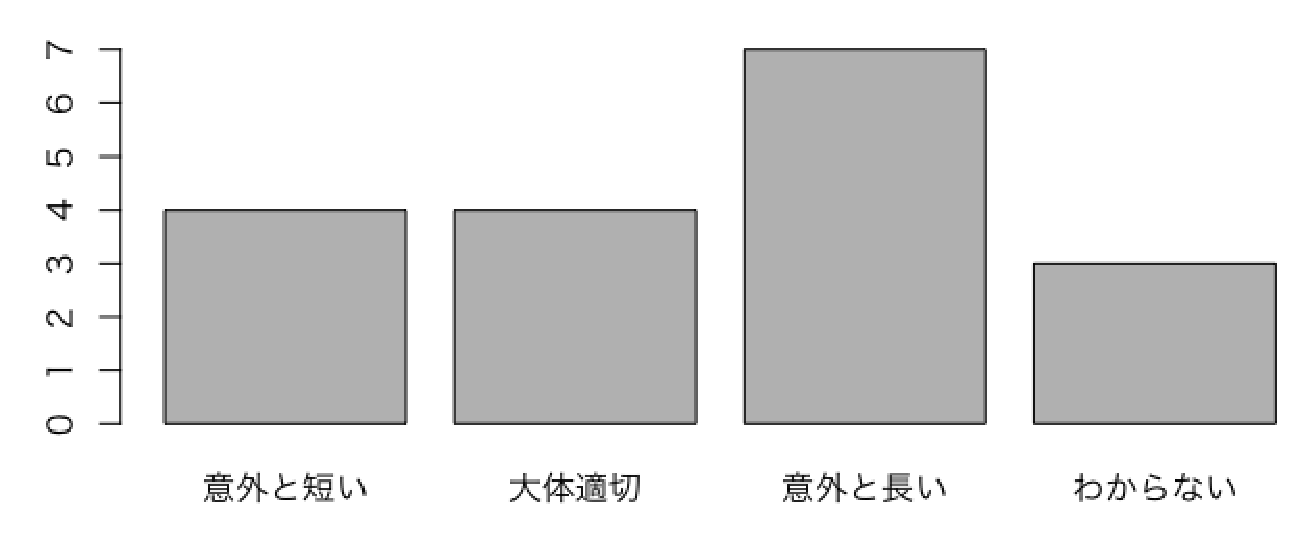
\includegraphics{data.eps}}
\end{center}
\caption{設問1の回答}
\label{fig:q1}
\end{figure}
この設問は見積り結果がどの程度の精度であると感じたかを調べるため実施したが,図\ref{fig:q1}より``意外と長い''が最も多い回答だった.
設問2``見積り結果はマネジメントに関して有用につかえましたか''という質問に対し,``はい''という回答が3件,``いいえ''が16件となった.
この設問は見積り結果がプロジェクトで実際に活用されたか否かを調べるため実施した.
設問3では設問2の回答結果に関して理由を質問した.
その結果,``気にしていなかった''という意見が最も多かった.
また設問4``見積り結果の発表タイミングはどうでしたか''の回答として,``わからない''が9件,``ちょうどいい''が5件,``遅すぎる''が5件となった.
これらに加え,GitHub運用ルールに対する感想をアンケートにて収集した.

\subsubsection{アンケート結果の考察} \label{quest-cons}
\ref{quest-detail}節の結果より,各回答をチームごとに分割して検証した.
その結果,各チームごとに設問4への回答に傾向が見られた.
例えばチームDとチームEのメンバーのうち3分の2が``遅すぎる''と回答しており,逆にチームEはメンバー全員が``ちょうどいい''と回答していた.
これは見積り結果発表時点での各チームの進捗状況の差が原因と考えられ,実際にチームD・Eで``遅すぎる''と回答したメンバーの過半数は,設問5で``見積り結果がほしい時期とずれていた''という旨の記述を行っていた.
この実験では全チームのデータを集め終わった段階で見積りを行った.
しかし,今後見積りを行う場合は,データが収集できたチームから順次見積りとその結果の通知を行う必要があることがわかった.

見積り結果が有効に使えたかの理由を聞いた設問3では,本来どのような目的で見積り結果を利用したかを確認するため実施したが,回答結果では``気にしていなかった''が最も多くなった.
同様に結果開示のタイミングが早かったか遅かったかを聞いた設問4では,``わからない''が最も多くなった.
これらの結果より今回の実験では多くの参加者が見積り結果に関してあまり関心を示していなかったことが分かった.
そのため,特にPBLを対象に見積りを行う場合,見積り結果の扱い方に関して事前により詳しく説明をする必要がある.

またGitHub運用ルールのうち``Issue発行ルール''が最も手間になったと回答され,この回答の半数以上が``他の方法で情報共有ができていたから不要だった''という旨を回答していた.
そのため,データの収集方法やPBLの運用方法を改めるなどの対策を行う必要があると考えられる.

%------------------------------------------------------------------------------
\section{結論} \label{conclusion}
\subsection{まとめ} \label{summary}
本研究はCoBRA法をベースにしたPBL向け工数見積り手法を提案し,進行中PBLへの適用実験を行った.
実験では必要データの収集を用意にするためプロジェクト管理ツールの運用ルールを指示してPBLを進行させた.
結果対象プロジェクトの多くでは一定の精度で工数を見積ることができた.
しかし,プロジェクトごとに開発の進捗に違いがあったため,適切なタイミングで見積り結果を提供できないプロジェクトが複数出てしまった.
また算出した見積り結果の扱い方について説明が足らず,有効に活かされなかった.
だが工数変動要因を収集するために設定したGitHub運用ルールによって,情報が見つけやすくなったなどの意見が得られた.

\subsection{今後の展望} \label{future-view}
本研究では,PBLのマネジメント支援のためにどの程度の見積り精度が必要であるかを調べられていないため,実施中のPBLを対象としたさらなる評価実験が必要である.
またPBLが担当教員や参加者が利用できるように提案手法のツール化が必要である.

%
%\begin{adjustvboxheight} % needed only when Appendix follows
\begin{thebibliography}{99}
\bibitem{pbl} ``PBLを基軸とする工学教育プログラム|九州工業大学.'' [Online]. Available: \url{http://www.mns.kyutech.ac.jp/~nakao-m/pbl/about.html.} [Accessed: 28-Dec-2016].
\bibitem{nagata2011} 永田佑輔 and 山戸昭三, ``1706 PBLで発生した問題とその解決事例(一般セッション),'' プロジェクトマネジメント学会研究発表大会予稿集, vol. 2011, pp. 504-506, Mar. 2011.
\bibitem{mastuzawa2009} 松澤芳昭, 塩見彰睦, 秡川友宏, and 酒井三四郎, ``ソフトウェア開発の教員主導型PBLにおける反復プロセスとEVM導入の効果,'' 研究報告コンピュータと教育(CE), vol. 2009-CE-99, no. 9, pp. 1-8, May 2009.
\bibitem{FP} 岡村正司, ``ファンクション・ポイント(IFP),'' in プロジェクトコスト見積もり入門:ファンクション・ポイント、COCOMOI\hspace{-1pt}I、WBSによるソフトウエア開発コストの導き方, 1st ed., 日経BP社, 2009, pp. 87-116.
\bibitem{ipa-web} ``エンタプライズ系事業/見積もり手法:IPA 独立行政法人 情報処理推進機構.'' [Online]. Available: \url{http://www.ipa.go.jp/sec/softwareengineering/std/ent01-c.html.} [Accessed: 25-Dec-2016].
\bibitem{yashima2011} 八島亮平, 山戸昭三, and 和田耕一, ``1202 Project Based Learningにおける見積もり手法に関する考察: ユースケースポイント法の適用(一般セッション),'' プロジェクトマネジメント学会研究発表大会予稿集, vol. 2011, pp. 99-102, Sep. 2011. 
\bibitem{CoBRA} Adam Trendowicz, Jens Heidrich, Jurgen Munch, Yasushi Ishigai, Kenji Yokoyama, Nahomi Kikuchi, ``Development of a hybrid cost estimation model in an iterative manner,'' ICSE 2006: 331-340.
\bibitem{enPiT2016} ``enPiT 分野・地域を越えた実践的情報教育協働ネットワーク.'' [Online]. Available: \url{http://www.enpit.jp/.} [Accessed: 15-Dec-2016].
\bibitem{github} ``Build software better, together,'' GitHub. [Online]. Available: \url{https://github.com.} [Accessed: 29-Dec-2016].
\bibitem{ogata1999} 緒方裕光 and 柳井晴夫, 統計学:基礎と応用, 初版. 京都: 現代数学社, 1999.
\end{thebibliography}
%\end{adjustvboxheight} % needed only when Appendix follows

%\appendix
%\subsection{付録: \LaTeX による論文作成のガイド} 
\begin{choshashoukai}

%\chosha{上田和紀}
%{1978年東京大学工学部計数工学科卒.
%1986年同大学大学院情報工学博士課程修了.
%工学博士.1983年NEC入社.
%1985年〜1992年 (財) 新世代コンピュータ技術開発機構出向.
%1993年より早稲田大学理工学部情報学科.
%現在,同理工学術院情報理工学科教授.
%プログラミング言語,並行・並列計算,高性能検証などの研究および
%システム開発に従事.
%第7回日本IBM科学賞,日本ソフトウェア科学会第4,5回論文賞など受賞.
%2004〜2007年度本誌編集委員長.}

\chosha{齋藤尊}
{2015年公立はこだて未来大学システム情報科学部情報アーキテクチャ学科卒.
2017年公立はこだて未来大学大学院システム情報科学研究科博士前期課程修了.
同年富士通株式会社入社.
}

\chosha{新美 礼彦}
{2002年桐蔭横浜大学大学院博士後期課程制御システム工学専攻修了(博士(工学)).
同年公立はこだて未来大学システム情報科学部助手.
%2004年同学科講師.
2009年より同大学准教授.
データマイニングに関する研究に従事.IEEE-CS, IEEE-SMC, 情報処理学会,人工知能学会,日本知能情報ファジィ学会各会員.}

\chosha{伊藤恵}
{1998 年北陸先端科学技術大学院大学情報科学研究科博士後期課程修了.
同年同研究科助手.
2001年公立はこだて未来大学講師.
2013年同大学准教授.
ソフトウェア科学会,情報処理学会,教育システム情報学会,観光情報学会,IEEE CS 各会員.}

\end{choshashoukai}

\end{document}
